\centerline{\bf \Huge Тренировочная олимпиада}
\centerline{\bf \Huge 9 класс}

\begin{flushright}
        \scriptsize{Завтра на сессии задачи будут сложнее}
\end{flushright}

\problem{1}
Арбуз и АрбузАрбуз по очереди вычеркивают по одному числу из ряда $1, 2, 3,\ldots, 2025$ до тех пор, пока не останется два числа. Если сумма этих чисел делится на $6$, то выигрывает Арбуз, если нет — АрбузАрбуз. Кто выиграет при правильной игре?

\problem{2}
Рассмотрим на плоскости прямоугольную решётку. Все вертикальные линии повернём на некоторый угол (см. рисунок). Назовём такую решётку \textit{косоугольной}. Назовём параллелограмм с вершинами в узлах решётки \textit{фундаментальным}, если он не содержит узлов внутри себя и на границах(кроме самих вершин). Докажите, что для любой конкретной косоугольной решётки все фундаментальные параллелограммы имеют одинаковые площади.

\begin{center}
    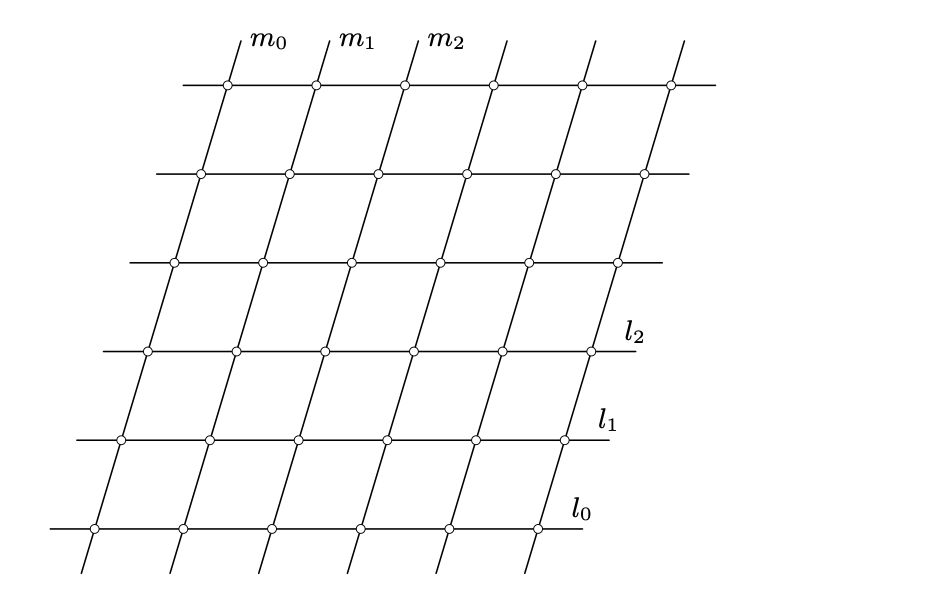
\includegraphics[width=0.6\textwidth]{ЭлМШ 2024-2025/IV блок/Тапиры/Olymp_9.png}
\end{center}

\problem{3}
Натуральные числа $a,b$ и $n$ таковы, что $a-b$ делится на $n$ и $ab$ делится на $n!$. Докажите, что об числа $a$ и $b$ делятся на $n$.


\problem{4}
Вневписанные окружности треугольника $A B C$ касаются его сторон $B C, C A$ и $A B$ в точках $A_1, B_1$ и $C_1$ соответственно. Точка $A$ лежит на окружности, описанной около треугольника $A_1 B_1 C_1$. Докажите, что вторая точка пересечения этой окружности со стороной $B C$ - основание высоты треугольника $A B C$, опущенной из вершины $A$.


\problem{5}
Существуют ли такие $a,b,c$ такие, что $|a| = |b| = |c| = |d|$ и уравнение $ax^3 + bx^2 + cx + d = 0$ имеет три различных корня?